\section{Analysis of first excitons in bulk hBN} \label{app:exc}
%
In bulk hBN due to the strong exciton localization the three fold symmetry cannot be disregarded and this makes the usual hydrogenic model inadequate to describe exciton series.\cite{attaccalite2018two}
Therefore we analyze the nature of the first excitons in bulk hBN using the solution of the full Bethe-Salpeter equation. Our analysis is based on direct comparison of exciton wave-functions with the results of Refs. \cite{paleari2018excitons,galvani2016excitons,attaccalite2018two}. By means of this comparison we were able  to recognize different excitonic states. However for a deeper analysis a tight-binding model and the plot of exciton phase is necessary \cite{galvani2016excitons} that is beyond the scope of this manuscript. In Table~\ref{exc_table} we report the first 13 excitonic states. For each state we report its binding energy both in self-consistent GW and G$_0$W$_0$ approximation, its symmetry, and the character inter-layer (IL) or in-plane pair (IP), using the same notation than  Ref. \cite{galvani2016excitons}. All these excitons are formed by $\pi \rightarrow \pi^*$ transition, that correspond to an hopping from nitrogen atom to the boron. For this reason the excitonic wave-function in Table~\ref{exc_table} are obtained by putting the hole on top of a nitrogen atom. Similar to the bi-layer case\cite{galvani2016excitons} in bulk h-BN excitons undergo to a Davydov splitting in even(\emph{grade}) and odd(\emph{ungrade}) states with respect to the inversion symmetry. The parity respect to the inversion symmetry is important for optical properties because transitions are allowed only with odd parity states.\cite{attaccalite2018two} This parity cannot be inferred from the plot of electron density at fixed hole position as in the figures of Table~\ref{exc_table} but requires an analysis of the exciton wave-function phase. Therefore we assigned parity by looking at the dipole matrix elements.
The first excitonic states from 1 to 4 correspond to the 1s exciton split in two degenerate pairs, already discussed in the text. Then we found a series of excitons similar to the monolayer case\cite{paleari2018excitons}: two with A$_1$ and $A_2$ symmetry, followed by a pair with E symmetry. At higher energy we have inter-layer excitons and then the degenerate states 12,13 that are the fist pair responsible for the second peak in the absorption spectra. At higher energy identification is more difficult but we expect to find all the Davydov pair the lowest excitons presented here.	
\begin{figure}[t]
\centering
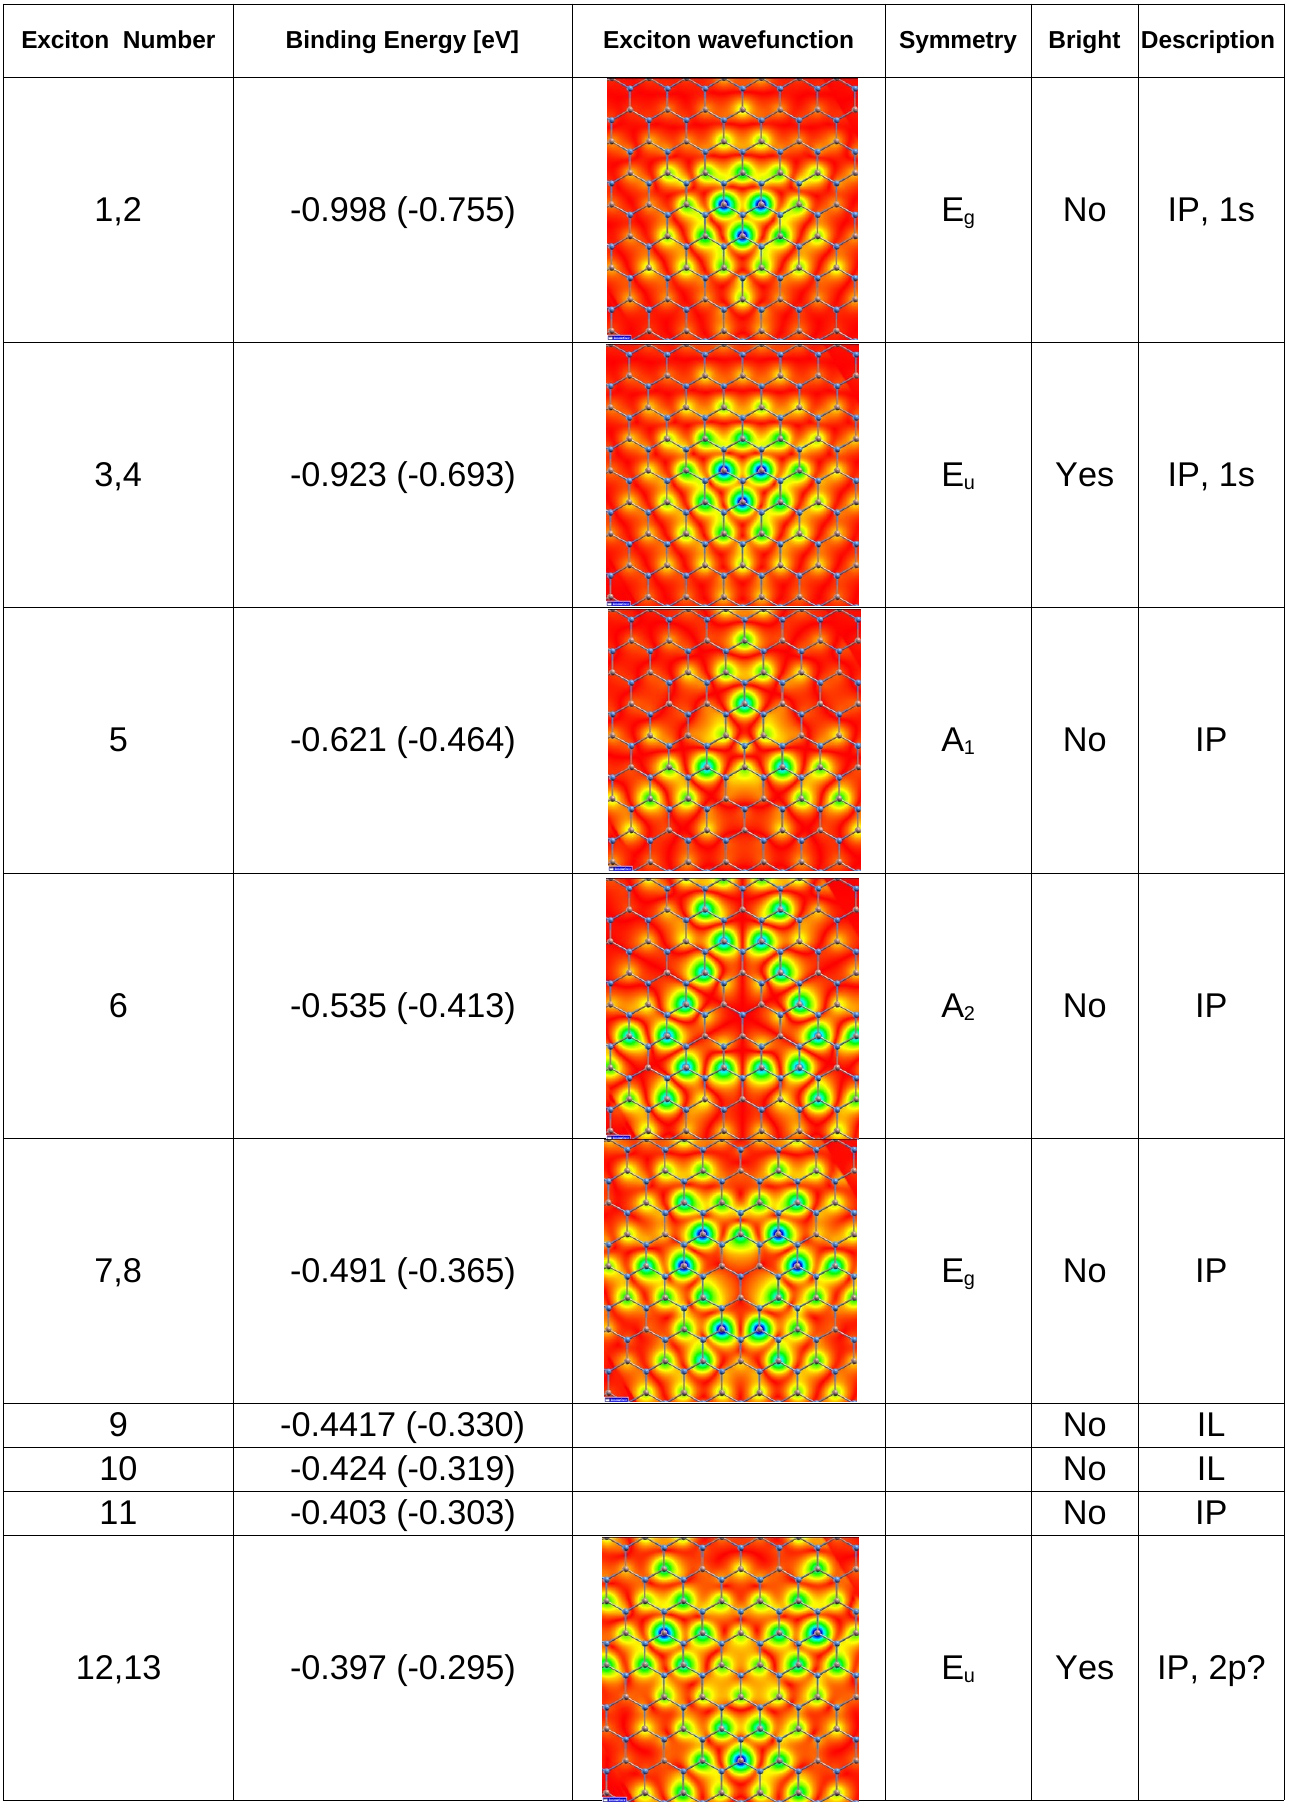
\includegraphics[height=0.9\textheight]{excitons.png}
    \caption{\footnotesize{The first 13 excitons in bulk hexagonal boron nitride. In this table we report both the binding energy in evGW and in G$_0$W$_0$ approximation.\label{exc_table}}}
\end{figure}